\documentclass[12pt]{article}
\usepackage{subfig}
\usepackage[margin=1in]{geometry}
\usepackage{amsmath,amsthm,amssymb}
\usepackage{graphicx}
\usepackage{subfigure}
\usepackage[figurename = Fig.]{caption}
%\usepackage{subcaption}
\newcommand{\N}{\mathbb{N}}
\newcommand{\R}{\mathbb{R}}
\newcommand{\Z}{\mathbb{Z}}
\newcommand{\Q}{\mathbb{Q}}
 \newcommand{\indep}{\rotatebox[origin=c]{90}{$\models$}}
\newenvironment{theorem}[2][Theorem]{\begin{trivlist}
\item[\hskip \labelsep {\bfseries #1}\hskip \labelsep {\bfseries #2.}]}{\end{trivlist}}
\newenvironment{lemma}[2][Lemma]{\begin{trivlist}
\item[\hskip \labelsep {\bfseries #1}\hskip \labelsep {\bfseries #2.}]}{\end{trivlist}}
\newenvironment{exercise}[2][Exercise]{\begin{trivlist}
\item[\hskip \labelsep {\bfseries #1}\hskip \labelsep {\bfseries #2.}]}{\end{trivlist}}
\newenvironment{problem}[2][Problem]{\begin{trivlist}
\item[\hskip \labelsep {\bfseries #1}\hskip \labelsep {\bfseries #2.}]}{\end{trivlist}}
\newenvironment{question}[2][Question]{\begin{trivlist}
\item[\hskip \labelsep {\bfseries #1}\hskip \labelsep {\bfseries #2.}]}{\end{trivlist}}
\newenvironment{corollary}[2][Corollary]{\begin{trivlist}
\item[\hskip \labelsep {\bfseries #1}\hskip \labelsep {\bfseries #2.}]}{\end{trivlist}}
 
\begin{document}
 
\title{Assignment5}
\author{Rui Yin}
 
\maketitle

\begin{problem}{1}Probability\\
1.\\
$(a)$ $P(X,Y|Z)$ apply Bayer's rule =  $\frac{P(Z|X,Y)P(X,Y)}{\sum{P(X,Y|Z=z)P(Z = z)}} = \frac{P(Z|X,Y)P(X,Y)}{P(Z)}$\\
$(b)$ X is conditional independent of Y and Z vice versa if $P(X,Y,Z) = P(X|Z)P(Y|Z)P(Z) = P(X|Y,Z)P(Y|X,Z)P(Z)$\\
$(c)$ X, Y independent, $P(X|Y) = P(X) = \frac{P(X,Y)}{P(Y)}, P(X|Y, Z) =  \frac{P(X,Y,Z)}{P(Y,Z)} =P(X|Z) = \frac{P(X,Z)}{P(Z)}$ and $ P(Z|Y) = \frac{P(Z,Y)}{P(Y)}$ now, we can get $P(Z)$ \\
$(d)$ $P(Y|X,Z) * P(X|Z) = \frac{P(X,Y,Z)}{P(X,Z)}*\frac{P(X,Z)}{P(Z)} = \frac{P(X,Y,Z)}{P(Z)} = P(X,Y|Z)$ same as \\
$P(X|Y,Z)*P(Y|Z) = \frac{P(X,Y,Z)}{P(Y,Z)}*\frac{P(Y,Z)}{P(Z)}=P(X,Y,Z)/P(Z) = P(X,Y|Z)$ and\\
$P(Y|X) = P(Y)$ because of conditional dependent, then $P(X|Z) = P(X)$\\
2.\\
$(a)$ in z condition x have union to y $X\indep $ Y\\
$(b)$ no $\indep$ because left equations means in y condition probability of x, then in right equation, there is in x condition probability of y, that's mean x, and y are dependent.\\
$(c)$ $X\indep $ Y\\
$(d)$ no  $\indep$ this is chain rule\\
3.\\
(a) $P(X|Y,Z) = \frac{P(X,Y|Z)}{P(Y|Z)} =$ chain rule$P(Z,Y,X) = P(Z)*P(Y|Z)*P(X|Y,Z) = \frac{\sum{X,Y,Z,w}}{\sum{Y,Z,w}}$ \\
(b)$P(X|Z)*P(Y|Z) = P(X,Y|Z) => P(X|Z) = \frac{P(X,Y|Z)}{P(Y|Z)} $\\

\end{problem}

\begin{problem}{2}Game Tree Search\\
(1)D:-11 E:-2 F:11 G:10, B:-2 C: 11 A:-2\\
(2) round1: D:-11, B:-11, A:-11, round2: E:-2, B:-2, A:-2 no pruned, because -2$>$-11\\
round3:F:11,C:11(pruned C)because of $-2<11$.\\
(3)no, if no purned we have to exam $b^d$ leaf nodes, where each node has b children, and d-play search if performed\\
(4)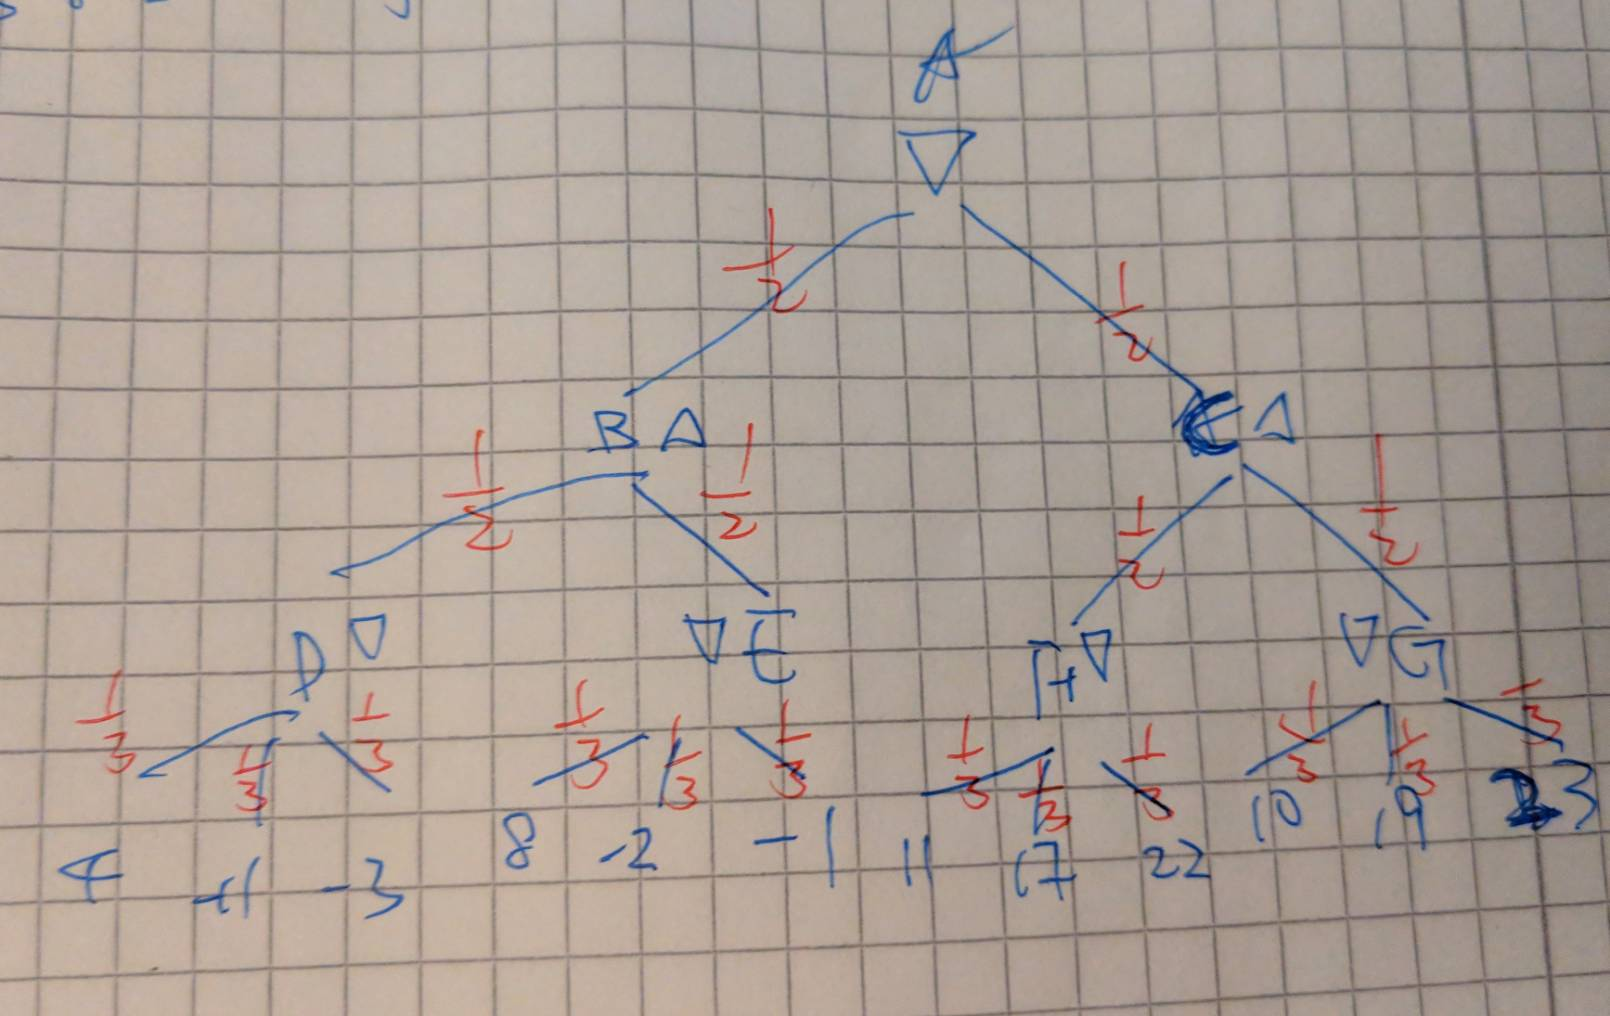
\includegraphics[width=7cm, height=4cm]{2.jpg}\\
(5)D:-3.3 E:-0.6 F:3.3, G:3.33,B:-1.65 C:1.65 A:0.83 \\

\end{problem}
\begin{problem}{3}Heuristic\\
(1)evaluate cost of cheapest path, h1 not admissible h(B)=14 $>$c(b,G)=12, h2:yes, all smaller or equal to h*.\\
(2)h1:ABCEDFG, h2:ABCDFEG, yes, they return different path. we sort all nodes to get the path order in forth step h1 and h2 chose E and D separately. \\
(3)$10\leq h_(D) \leq5.5 $\\
(4)$10\leq h_(D) \leq5.5 $ B and C not in sequential order,$h_3(B) < h_3(C)$ therefore C will be in front of B.\\
\end{problem}



\end{document}
